\documentclass[14pt,a4paper]{article}
\usepackage[14pt]{extsizes}
\usepackage[left=1.5cm, right=1.5cm, top=1.5cm, bottom=1.5cm]{geometry}
\usepackage[utf8]{inputenc}
\usepackage[T2A]{fontenc}
\usepackage[english, russian]{babel}
\usepackage{amsmath,amsfonts,amssymb,amsthm,mathtools} 
\usepackage{amsfonts}
\usepackage{amssymb}
\usepackage{titleps}
\usepackage{hyperref}
\usepackage{float}
\usepackage{graphicx}
\usepackage{multirow}
\usepackage{hhline}
\usepackage{wrapfig}
\usepackage{tikz}
\usepackage{pgfplots}
\usepackage{xcolor}
\usepackage{subfig}
\usepackage{upgreek}

\newcommand{\w}[1]{\text{#1}}
\newcommand{\und}[1]{\underline{#1}}
\newcommand{\img}[3]{
	\begin{figure}[H]
	\begin{center}
	\includegraphics[scale=#2]{#1}
	\end{center}
	\begin{center}
 	\textit{#3}
	\end{center}
	\end{figure}
}
\newcommand{\aw}[1]{
	\begin{center}
	\textit{#1}
	\end{center}
	\n
}
\newcommand{\be}[1]{
	\begin{center}
	\boxed{#1}
	\end{center}
}
\newcommand{\beb}[1]{
	\begin{equation}
	\boxed{#1}
	\end{equation}
}
\newcommand{\eb}[1]{
	\begin{equation}
	#1
	\end{equation}
}
\newcommand{\n}{\hfill \break}
\newcommand{\x}{\cdot}

\begin{document}

\section*{Работа 3.3.4}	
\section*{Эффект Холла в полупроводниках}
\subsection*{Киркича Андрей, Б01-202, МФТИ}
\n
\textbf{Цель работы:} измерение подвижности и концентрации носителей заряда в полупроводниках.
\n\n
\textbf{В работе используются:} электромагнит с источником питания, амперметр, миллиамперметр, милливеберметр, реостат, цифровой вольтметр, источник питания (1.5 В), образцы легированного германия.


\section*{Теоретические сведения}

Пусть через однородную пластину металла вдоль оси $ x $ течёт ток $ I $. Если эту пластину поместить в магнитное поле, направленное по оси $ y $, то между гранями А и Б появляется разность потенциалов.

\begin{wrapfigure}{r}{6cm}
	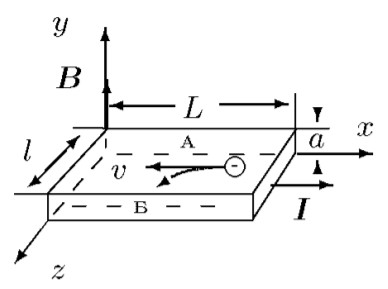
\includegraphics[width=6cm]{holl.jpg}
	\caption{Образец с током в магнитном поле}
	\label{ris1}
	\vspace{1.5cm}
\end{wrapfigure}

\n
В самом деле, на электрон, движущийся со скоростью $ \left\langle \bm{v} \right\rangle $ в электромагнитном поле, действует сила Лоренца:
\[ \bm{F_{\text{Л}}} = -e \bm{E} - e \left\langle \bm{v} \right\rangle \times \bm{B} ,\]

где $ e $ -- абсолютная величина заряда электрона, $ \bm{E} $ -- напряжённость электрического поля, $ \bm{B} $ -- индукция магнитного поля. В нашем случае сила, обусловленная вторым слагаемым, направлена вдоль оси $ z $:
\[ F_B = e |\left\langle v_x \right\rangle| B. \]
\n
В данной формуле $ |\left\langle v_x \right\rangle| $ -- абсолютная величина дрейфовой скорости электронов вдоль оси $ x $. Электроны отклоняются к грани Б, на грани А накапливаются нескомпенсированные положительные заряды. Это приводит к возникновению электрического поля $ E_z $, направленного от А к Б, которое действует на электроны с силой $ F_E=eE_z $, направленной против силы $ F_B $. В установившемся режиме сила $ F_E $ уравновешивает силу $ F_B $, из условия равновесия имеем:
\[ E_z = |\left\langle v_x \right\rangle| B. \]
\n
Поле $ E_z $ даёт вклад в общее поле $ \bm{E} $, в котором движутся электроны. С полем $ E_z $ связана разность потенциалов $ U_\text{АБ} = -E_z l = - |\left\langle v_x \right\rangle| B l.$ В этом и состоит эффект Холла. Замечая, что сила тока  I = $n e |\left\langle v_x \right\rangle| l a $, получаем ЭДС Холла:

\begin{equation}\label{1}
\mathcal{E}_x = U_\text{АБ}= - \frac{IB}{nea} = - R_x \cdot \frac{IB}{a}, \qquad R_x=\frac{1}{ne}.
\end{equation}
\n
Константа $ R_x $ называется постоянной Холла.

\section*{Экспериментальная установка}

\begin{figure}[h]
	\centering
	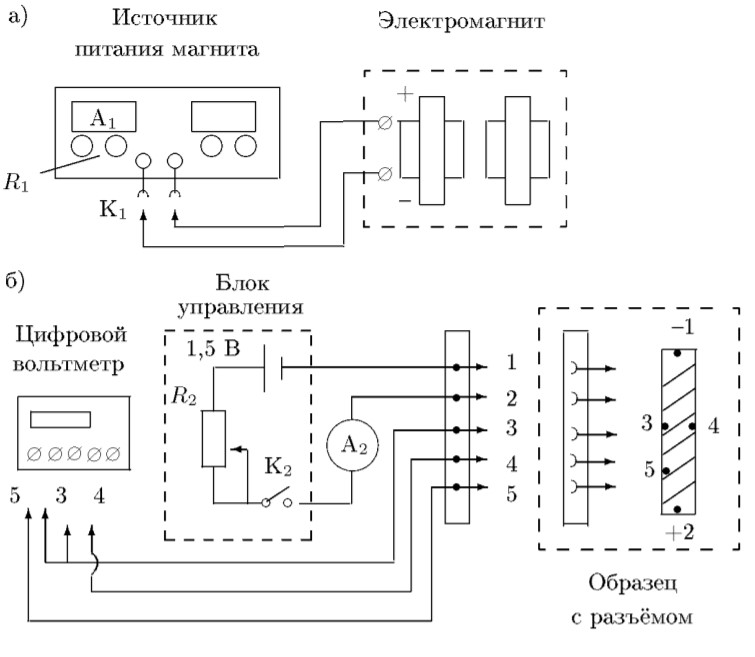
\includegraphics[width=15cm]{ust.jpg}
	\caption{Схема установки для исследования эффекта Холла	в полупроводниках}
	\label{ust}
\end{figure}

\n
ЭДС Холла можно рассчитать следующим образом:
\[\mathcal{E}_x = U_{34} \pm U_0,\]

где $U_0$ - омическое падение напряжения, вызванное протеканием тока через образец, $U_{34}$ - напряжение между точками 3 и 4.
\n\n
По знаку $ \mathcal{E} $ можно определить характер проводимости -- электронный или дырочный. Для этого необходимо знать направление тока в образце и направление магнитного поля.
\n\n
Измерив ток $ I $ в образце и напряжение $ U_{35} $ между контактами 3 и 5 в отсутствие магнитного поля, можно рассчитать проводимость материала образца по формуле:
\begin{equation}\label{2}
\sigma = \frac{IL_{35}}{U_{35}al},
\end{equation}

где $ L_{35} $ -- расстояние между контактами 3 и 5, $ a $ -- толщина образца, $ l $ -- его ширина.

\section*{Обработка результатов измерений}

\subsection*{Градуировка электромагнита}

При помощи тесламетра мы изучили зависимость величины магнитной индукции между полюсами прибора от тока в катушках электромагнита. Результаты измерений представлены в таблице. Погрешности: $ \quad \sigma_{I} = 0,2$ А, $ \quad \sigma_{B} = 20$ мТл.

\begin{table}[H]
	\centering
	\begin{tabular}{|l|r|r|r|r|r|r|r|r|r|r|r|r|r|r|}
		\hline
		$ I_\text{м} $, А & 0,1 & 0,2 & 0,3 & 0,4 & 0,5 & 0,6 & 0,7 & 0,8 & 0,9 & 1,0 & 1,1 & 1,2 & 1,3 & 1,4 \\ \hline
		$ B $, мТл & 110 & 200 & 320 & 430 & 530 & 630 & 720 & 800 & 870 & 910 & 950 & 990 & 1030 & 1050 \\ \hline
	\end{tabular}
\end{table}
\subsection*{Измерение ЭДС Холла}

Для разных значений $ I $ через образец была снята зависимость ЭДС Холла от тока $ I_\text{м} $ через электромагнит. Результаты измерений мы занесли в таблицу ниже. Погрешности измерений: $ \quad \sigma_{I} = 0,2$ А, $ \quad \sigma_{U} = 0,02$ мВ.

\begin{longtable}[c]{l|rr|rr|rr|}
		\hline
		\multicolumn{1}{|c|}{$I$, мА}   & \multicolumn{2}{r|}{0,2}                      & \multicolumn{2}{r|}{0,3}                      & \multicolumn{2}{r|}{0,4}                      \\ \hline
		\multicolumn{1}{|c|}{$U_0$, мВ} & \multicolumn{2}{r|}{-0,02}                    & \multicolumn{2}{r|}{-0,06}                    & \multicolumn{2}{r|}{-0,07}                    \\ \hline
		\multicolumn{1}{r|}{}           & \multicolumn{1}{r|}{$I_\text{м}$, А} & $U$, мВ & \multicolumn{1}{c|}{$I_\text{м}$, А} & $U$, мВ & \multicolumn{1}{c|}{$I_\text{м}$, А} & $U$, мВ \\ \cline{2-7} 
		\multicolumn{1}{r|}{}           & \multicolumn{1}{r|}{0,2}            & -0,05  & \multicolumn{1}{r|}{0,2}            & -0,11  & \multicolumn{1}{r|}{0,2}            & -0,15  \\ \cline{2-7} 
		\multicolumn{1}{r|}{}           & \multicolumn{1}{r|}{0,4}            & -0,08  & \multicolumn{1}{r|}{0,4}            & -0,17  & \multicolumn{1}{r|}{0,4}            & -0,23  \\ \cline{2-7} 
		\multicolumn{1}{r|}{}           & \multicolumn{1}{r|}{0,6}            & -0,10  & \multicolumn{1}{r|}{0,6}            & -0,23  & \multicolumn{1}{r|}{0,6}            & -0,31  \\ \cline{2-7} 
		\multicolumn{1}{r|}{}           & \multicolumn{1}{r|}{0,8}            & -0,13  & \multicolumn{1}{r|}{0,8}            & -0,27  & \multicolumn{1}{r|}{0,8}            & -0,37  \\ \cline{2-7} 
		\multicolumn{1}{r|}{}           & \multicolumn{1}{r|}{1,0}            & -0,14  & \multicolumn{1}{r|}{1,0}            & -0,31  & \multicolumn{1}{r|}{1,0}            & -0,41  \\ \cline{2-7} 
		\multicolumn{1}{r|}{}           & \multicolumn{1}{r|}{1,2}            & -0,15  & \multicolumn{1}{r|}{1,2}            & -0,33  & \multicolumn{1}{r|}{1,2}            & -0,44  \\ \cline{2-7} 
		\multicolumn{1}{r|}{}           & \multicolumn{1}{r|}{1,4}            & -0,16  & \multicolumn{1}{r|}{1,4}            & -0,35  & \multicolumn{1}{r|}{1,4}            & -0,47  \\ \hline
		\multicolumn{1}{|c|}{$I$, мА}   & \multicolumn{2}{r|}{0,5}                      & \multicolumn{2}{r|}{0,6}                      & \multicolumn{2}{r|}{0,7}                      \\ \hline
		\multicolumn{1}{|c|}{$U_0$, мВ} & \multicolumn{2}{r|}{-0,09}                    & \multicolumn{2}{r|}{-0,11}                    & \multicolumn{2}{r|}{-0,13}                    \\ \hline
		& \multicolumn{1}{c|}{$I_\text{м}$, А} & $U$, мВ & \multicolumn{1}{c|}{$I_\text{м}$, А} & $U$, мВ & \multicolumn{1}{c|}{$I_\text{м}$, А} & $U$, мВ \\ \cline{2-7} 
		& \multicolumn{1}{r|}{0,2}            & -0,20  & \multicolumn{1}{r|}{0,2}            & -0,23  & \multicolumn{1}{r|}{0,2}            & -0,28  \\ \cline{2-7} 
		& \multicolumn{1}{r|}{0,4}            & -0,29  & \multicolumn{1}{r|}{0,4}            & -0,35  & \multicolumn{1}{r|}{0,4}            & -0,41  \\ \cline{2-7} 
		& \multicolumn{1}{r|}{0,6}            & -0,38  & \multicolumn{1}{r|}{0,6}            & -0,46  & \multicolumn{1}{r|}{0,6}            & -0,54  \\ \cline{2-7} 
		& \multicolumn{1}{r|}{0,8}            & -0,46  & \multicolumn{1}{r|}{0,8}            & -0,56  & \multicolumn{1}{r|}{0,8}            & -0,65  \\ \cline{2-7} 
		& \multicolumn{1}{r|}{1,0}            & -0,52  & \multicolumn{1}{r|}{1,0}            & -0,62  & \multicolumn{1}{r|}{1,0}            & -0,73  \\ \cline{2-7} 
		& \multicolumn{1}{r|}{1,2}            & -0,56  & \multicolumn{1}{r|}{1,2}            & -0,67  & \multicolumn{1}{r|}{1,2}            & -0,79  \\ \cline{2-7} 
		& \multicolumn{1}{r|}{1,4}            & -0,58  & \multicolumn{1}{r|}{1,4}            & -0,71  & \multicolumn{1}{r|}{1,4}            & -0,83  \\ \hline
		\multicolumn{1}{|c|}{$I$, мА}   & \multicolumn{2}{r|}{0,8}                      & \multicolumn{2}{r|}{1,0}                      & \multicolumn{2}{r|}{1,0 (обр.)}                      \\ \hline
		\multicolumn{1}{|c|}{$U_0$, мВ} & \multicolumn{2}{r|}{-0,16}                    & \multicolumn{2}{r|}{-0,19}                    & \multicolumn{2}{r|}{-0,19 (обр.)}                    \\ \hline
		& \multicolumn{1}{c|}{$I_\text{м}$, А} & $U$, мВ & \multicolumn{1}{c|}{$I_\text{м}$, А} & $U$, мВ & \multicolumn{1}{c|}{$I_\text{м}$, А} & $U$, мВ \\ \cline{2-7} 
		& \multicolumn{1}{r|}{0,2}            & -0,31  & \multicolumn{1}{r|}{0,2}            & -0,40  & \multicolumn{1}{r|}{0,2}            & 0,00   \\ \cline{2-7} 
		& \multicolumn{1}{r|}{0,4}            & -0,48  & \multicolumn{1}{r|}{0,4}            & -0,56  & \multicolumn{1}{r|}{0,4}            & 0,21   \\ \cline{2-7} 
		& \multicolumn{1}{r|}{0,6}            & -0,62  & \multicolumn{1}{r|}{0,6}            & -0,77  & \multicolumn{1}{r|}{0,6}            & 0,39   \\ \cline{2-7} 
		& \multicolumn{1}{r|}{0,8}            & -0,75  & \multicolumn{1}{r|}{0,8}            & -0,93  & \multicolumn{1}{r|}{0,8}            & 0,54   \\ \cline{2-7} 
		& \multicolumn{1}{r|}{1,0}            & -0,84  & \multicolumn{1}{r|}{1,0}            & -1,04  & \multicolumn{1}{r|}{1,0}            & 0,66   \\ \cline{2-7} 
		& \multicolumn{1}{r|}{1,2}            & -0,90  & \multicolumn{1}{r|}{1,2}            & -1,13  & \multicolumn{1}{r|}{1,2}            & 0,74   \\ \cline{2-7} 
		& \multicolumn{1}{r|}{1,4}            & -0,95  & \multicolumn{1}{r|}{1,4}            & -1,19  & \multicolumn{1}{r|}{1,4}            & 0,79   \\ \cline{2-7} 
\end{longtable}
\n
Последнее измерение было произведено при изменённой ориентации образца. Затем мы вычислили значение $ \mathcal{E}_x $ по разности показаний вольтметра и сопоставили токи в электромагните с соответствующими значениями индукции магнитного поля. Полученные результаты представлены ниже. Погрешности: $\quad \sigma_{B} = 20$ мТл, $\quad \sigma_{\mathcal{E}_x} = 0,03$ мВ.

% Please add the following required packages to your document preamble:
% \usepackage{longtable}
% Note: It may be necessary to compile the document several times to get a multi-page table to line up properly
\begin{longtable}[c]{c|rr|rr|rr|}
	\hline
	\multicolumn{1}{|c|}{$I$, мА} & \multicolumn{2}{r|}{0,2}                          & \multicolumn{2}{r|}{0,3}                          & \multicolumn{2}{r|}{0,4}                          \\ \hline
	\endfirsthead
	%
	\endhead
	%
	& \multicolumn{1}{c|}{$B$, мТл} & $\mathcal{E}_x$, мВ & \multicolumn{1}{c|}{$B$, мТл} & $\mathcal{E}_x$, мВ & \multicolumn{1}{c|}{$B$, мТл} & $\mathcal{E}_x$, мВ \\ \cline{2-7} 
	& \multicolumn{1}{r|}{200}   & 0,04               & \multicolumn{1}{r|}{200}  & 0,06               & \multicolumn{1}{r|}{200}   & 0,08               \\ \cline{2-7} 
	& \multicolumn{1}{r|}{430}   & 0,07               & \multicolumn{1}{r|}{430}   & 0,12               & \multicolumn{1}{r|}{430}   & 0,16               \\ \cline{2-7} 
	& \multicolumn{1}{r|}{630}   & 0,08               & \multicolumn{1}{r|}{630}   & 0,18               & \multicolumn{1}{r|}{630}   & 0,24               \\ \cline{2-7} 
	& \multicolumn{1}{r|}{800}   & 0,11               & \multicolumn{1}{r|}{800}   & 0,22               & \multicolumn{1}{r|}{800}   & 0,29               \\ \cline{2-7} 
	& \multicolumn{1}{r|}{910}   & 0,12               & \multicolumn{1}{r|}{910}   & 0,25               & \multicolumn{1}{r|}{910}   & 0,34               \\ \cline{2-7} 
	& \multicolumn{1}{r|}{990}   & 0,13               & \multicolumn{1}{r|}{990}   & 0,28               & \multicolumn{1}{r|}{990}   & 0,37               \\ \cline{2-7} 
	& \multicolumn{1}{r|}{1050}  & 0,14               & \multicolumn{1}{r|}{1050}  & 0,29               & \multicolumn{1}{r|}{1050}  & 0,39               \\ \hline
	\multicolumn{1}{|c|}{$I$, мА} & \multicolumn{2}{r|}{0,5}                          & \multicolumn{2}{r|}{0,6}                          & \multicolumn{2}{r|}{0,7}                          \\ \hline
	& \multicolumn{1}{c|}{$B$, мТл} & $\mathcal{E}_x$, мВ & \multicolumn{1}{c|}{$B$, мТл} & $\mathcal{E}_x$, мВ & \multicolumn{1}{c|}{$B$, мТл} & $\mathcal{E}_x$, мВ \\ \cline{2-7} 
	& \multicolumn{1}{r|}{200}   & 0,11               & \multicolumn{1}{r|}{200}   & 0,12               & \multicolumn{1}{r|}{200}   & 0,14               \\ \cline{2-7} 
	& \multicolumn{1}{r|}{430}   & 0,20               & \multicolumn{1}{r|}{430}   & 0,24               & \multicolumn{1}{r|}{430}   & 0,28               \\ \cline{2-7} 
	& \multicolumn{1}{r|}{630}   & 0,29               & \multicolumn{1}{r|}{630}   & 0,35               & \multicolumn{1}{r|}{630}   & 0,40               \\ \cline{2-7} 
	& \multicolumn{1}{r|}{800}   & 0,37               & \multicolumn{1}{r|}{800}   & 0,44               & \multicolumn{1}{r|}{800}   & 0,52               \\ \cline{2-7} 
	& \multicolumn{1}{r|}{910}   & 0,42               & \multicolumn{1}{r|}{910}   & 0,51               & \multicolumn{1}{r|}{910}   & 0,60               \\ \cline{2-7} 
	& \multicolumn{1}{r|}{990}   & 0,46               & \multicolumn{1}{r|}{990}   & 0,56               & \multicolumn{1}{r|}{990}   & 0,65               \\ \cline{2-7} 
	& \multicolumn{1}{r|}{1050}  & 0,49               & \multicolumn{1}{r|}{1050}  & 0,59               & \multicolumn{1}{r|}{1050}  & 0,69               \\ \hline
	\multicolumn{1}{|c|}{$I$, мА} & \multicolumn{2}{r|}{0,8}                          & \multicolumn{2}{r|}{1,0}                          & \multicolumn{2}{r|}{1,0 (обр.)}                \\ \hline
	& \multicolumn{1}{c|}{$B$, мТл} & $\mathcal{E}_x$, мВ & \multicolumn{1}{c|}{$B$, мТл} & $\mathcal{E}_x$, мВ & \multicolumn{1}{c|}{$B$, мТл} & $\mathcal{E}_x$, мВ \\ \cline{2-7} 
	& \multicolumn{1}{r|}{200}   & 0,16               & \multicolumn{1}{r|}{200}   & 0,20               & \multicolumn{1}{r|}{200}   & 0,19               \\ \cline{2-7} 
	& \multicolumn{1}{r|}{430}   & 0,32               & \multicolumn{1}{r|}{430}   & 0,36               & \multicolumn{1}{r|}{430}   & 0,40               \\ \cline{2-7} 
	& \multicolumn{1}{r|}{630}   & 0,47               & \multicolumn{1}{r|}{630}   & 0,58               & \multicolumn{1}{r|}{630}   & 0,58               \\ \cline{2-7} 
	& \multicolumn{1}{r|}{810}   & 0,59               & \multicolumn{1}{r|}{800}   & 0,74               & \multicolumn{1}{r|}{800}   & 0,74               \\ \cline{2-7} 
	& \multicolumn{1}{r|}{910}   & 0,68               & \multicolumn{1}{r|}{910}   & 0,85               & \multicolumn{1}{r|}{910}   & 0,85               \\ \cline{2-7} 
	& \multicolumn{1}{r|}{990}   & 0,75               & \multicolumn{1}{r|}{990}   & 0,94               & \multicolumn{1}{r|}{990}   & 0,94               \\ \cline{2-7} 
	& \multicolumn{1}{r|}{1050}  & 0,79               & \multicolumn{1}{r|}{1050}  & 0,99               & \multicolumn{1}{r|}{1050}  & 0,99               \\ \cline{2-7} 
\end{longtable}

%
%По полученным данным построим графики зависимости $ \mathcal{E}_x(B) $ для различных значений $ I $.
%
%
%\begin{center}
%	\begin{tikzpicture}
%	\begin{axis}[
%	title={График 2 \quad Графики зависимости $ \mathcal{E}_x(B) $},
%	xlabel={$ B $, мТлл},
%	ylabel={$ \mathcal{E}_x $, мВ},
%	legend pos=north west,
%	xmajorgrids=true,
%	ymajorgrids=true,
%	grid style=dashed,
%	width = 520,
%	height = 380,
%	%xmin = 300,
%	%xmax = 335,
%	%ymin =40,
%	%ymax =135,
%	]
%	\legend{
%	$ I_\text{м}  = 0.15 $ мА,
%	$ I_\text{м}  = 0.30 $ мА,
%	$ I_\text{м}  = 0.40 $ мА,
%	$ I_\text{м}  = 0.50 $ мА,
%	$ I_\text{м}  = 0.60 $ мА,
%	$ I_\text{м}  = 0.70 $ мА,
%	$ I_\text{м}  = 0.80 $ мА,
%	$ I_\text{м}  = 1.00 $ мА,
%	$ I^{flip}_\text{м}  = 1.00 $ мА,,,,,,,,,};
%	\addplot+ [ only marks, mark size = 4pt, mark=*,
%	error bars/.cd,
%	x dir=both, x explicit,
%	y dir=both, y explicit, 
%	] table [x = T, y = sigma,] {
%		T	sigma               
%		202.9	0.028
%		428.1	0.058
%		632.3	0.083
%		801.1	0.107
%		914.3	0.123
%		992.3	0.133
%		1048.6	0.141
%	};
%	\addplot+ [ only marks, mark size = 4pt, mark=oplus*,
%	error bars/.cd,
%	x dir=both, x explicit,
%	y dir=both, y explicit, 
%	] table [x = T, y = sigma,] {
%		T	sigma               
%		202.9	0.060
%		428.1	0.118
%		632.3	0.175
%		801.1	0.221
%		914.3	0.254
%		992.3	0.276
%		1048.6	0.294
%	};
%	\addplot+ [ only marks, mark size = 4pt, mark=square*,
%	error bars/.cd,
%	x dir=both, x explicit,
%	y dir=both, y explicit, 
%	] table [x = T, y = sigma,] {
%		T	sigma               
%		202.9	0.084
%		428.1	0.158
%		632.3	0.236
%		801.1	0.297
%		914.3	0.342
%		992.3	0.372
%		1048.6	0.397	
%	};
%	\addplot+ [ only marks, mark size = 4pt, mark=triangle*,
%	error bars/.cd,
%	x dir=both, x explicit,
%	y dir=both, y explicit, 
%	] table [x = T, y = sigma,] {
%		T	sigma               
%		202.9	0.106
%		428.1	0.201
%		632.3	0.287
%		801.1	0.369
%		914.3	0.426
%		992.3	0.466
%		1048.6	0.493	
%	};
%	\addplot+ [ only marks, mark size = 4pt, mark=diamond*,
%	error bars/.cd,
%	x dir=both, x explicit,
%	y dir=both, y explicit, 
%	] table [x = T, y = sigma,] {
%		T	sigma               
%		202.9	0.124
%		428.1	0.240
%		632.3	0.351
%		801.1	0.448
%		914.3	0.515
%		992.3	0.563
%		1048.6	0.597	
%	};
%	\addplot+ [ only marks, mark size = 4pt, mark=halfdiamond*,
%	error bars/.cd,
%	x dir=both, x explicit,
%	y dir=both, y explicit, 
%	] table [x = T, y = sigma,] {
%		T	sigma               
%		202.9	0.147
%		428.1	0.285
%		632.3	0.409
%		801.1	0.522
%		914.3	0.602
%		992.3	0.658
%		1048.6	0.698	
%	};
%	\addplot+ [ only marks, mark size = 4pt, mark=halfsquare right*,
%	error bars/.cd,
%	x dir=both, x explicit,
%	y dir=both, y explicit, 
%	] table [x = T, y = sigma,] {
%		T	sigma               
%		202.9	0.162
%		428.1	0.325
%		632.3	0.470
%		801.1	0.596
%		914.3	0.687
%		992.3	0.751
%		1048.6	0.798	
%	};
%	\addplot+ [ only marks, mark size = 4pt, mark=pentagon*,
%	error bars/.cd,
%	x dir=both, x explicit,
%	y dir=both, y explicit, 
%	] table [x = T, y = sigma,] {
%		T	sigma               
%		202.9	0.207
%		428.1	0.368
%		632.3	0.585
%		801.1	0.744
%		914.3	0.850
%		992.3	0.941
%		1048.6	0.997
%	};
%	\addplot+ [ only marks, mark size = 4pt, mark=halfsquare left*,
%	error bars/.cd,
%	x dir=both, x explicit,
%	y dir=both, y explicit, 
%	] table [x = T, y = sigma,] {
%		T	sigma               
%		202.9	0.198
%		428.1	0.404
%		632.3	0.586
%		801.1	0.743
%		914.3	0.857
%		992.3	0.942
%		1048.6	0.991
%	};
%	\addplot [blue, domain=190:1100, line width =3.2pt] {0.0003192+0.0001336*x};
%	\addplot [red, domain=190:1100, line width =3.2pt] {0.0013500+0.0002766*x};
%	\addplot [brown, domain=190:1100, line width =3.2pt] {0.0035500+0.0003708*x};
%	\addplot [black, domain=190:1100, line width =3.2pt] {0.0056900+0.0004598*x};
%	\addplot [blue, domain=190:1100, line width =3.2pt] {0.0030700+0.0005611*x};
%	\addplot [red, domain=190:1100, line width =3.2pt] {0.0069800+0.0006519*x};
%	\addplot [brown, domain=190:1100, line width =3.2pt] {0.0038200+0.0007495*x};
%	\addplot [blue, domain=190:1100, line width =3.2pt] {-0.0108300+0.0009498*x};
%	\addplot [domain=190:1100, line width =3.2pt] {0.0009906+0.0009391*x};
%	\end{axis}
%	\end{tikzpicture}
%\end{center}
\n
Полученные данные были аппроксимированы зависимостями вида $  \mathcal{E}_x=K(I)B+c $. Результаты представлены в таблице. Погрешности: $ \quad \sigma_{I} = 0,2$ А, $ \quad \sigma_{K} = 30$ В/Тл.

\begin{table}[H]
	\centering
	\resizebox{0.9\textwidth}{!}{
	\begin{tabular}{|l|r|r|r|r|r|r|r|r|r|}
		\hline
		$ I $, мА & 0,2 & 0,3 & 0,4 & 0,5 & 0,6 & 0,7 & 0,8 & 0,9 & 1,0 \\ \hline
		$ K(I) $, В/Тл & 130 & 280 & 370 & 460 & 560 & 650 & 750 & 940 & 950 \\ \hline
	\end{tabular}
	}
\end{table}
\n
Аппроксимируя зависимость прямой вида $ K=pI $, получили:
\[p = (94\pm2) \cdot 10^{-2} \text{ } \frac{\text{В}}{\text{Тл}\cdot\text{А}}.\]
\n
Тогда, согласно \eqref{1}, $ R_x = pa $, где $ a = 1 $ мм -- толщина исследуемого образца. Имеем:
\[R_x = (94\pm9) \cdot 10^{-5} \text{ } \frac{\text{В}\cdot\text{м}}{\text{Тл}\cdot\text{А}}.\]
\n
Отсюда можно найти концентрацию носителей заряда:
\[n = (66\pm7) \cdot 10^{20} \text{ м}^{-3}.\]

\subsection*{Расчёт удельной проводимости и подвижности}

По результатам измерений $ U_{35} = (4,0 \pm 0,2) $ мВ, $ L_{35} = (5 \pm 1) $ мм и $ l = (4 \pm 1) $ мм. В итоге по формуле (2) получили:
\[\sigma = (310\pm20)\text{ } (\text{Ом}\cdot\text{м})^{-1}.\]
\n
Зная эти характеристики, можно рассчитать подвижность носителей заряда:
\[b=\frac{\sigma}{en} = (2900\pm300) \text{ } \frac{\text{см}^2}{\text{В}\cdot\text{с}}.\]

\section*{Заключение}

В ходе выполнения данной лабораторной работы был исследован эффект Холла в полупроводнике, а именно в легированном германии. Была определена постоянная Холла для исследуемого образца $ R_x = (94\pm9) \cdot 10^{-5} \frac{\text{В}\cdot\text{м}}{\text{Тл}\cdot\text{А}} $. Также была вычислена концентрация носителей заряда $ n = (66\pm7) \cdot 10^{20} \text{ м}^{-3}. $
\n\n
По полярности вольтметра, полярности подключения источника тока и направлению тока в катушках была определён тип проводимости - электронный.
\n\n
Также была вычислена подвижность электронов германия: $ b = (2900\pm300) \text{ } \frac{\text{см}^2}{\text{В}\cdot\text{с}} $. Однако полученный результат отличается от табличной подвижности электронов в германии: $ b_{\text{табл}} = 3900 \text{ } \frac{\text{см}^2}{\text{В}\cdot\text{с}} $. Это может свидетельствовать о наличии примесей исследуемом образце.
\n\n
Также ощутимый вклад в ошибку полученных данных может внести зависимость характеристик исследуемого образца от температуры, которая могла значительно изменяться в силу прохождения через образец электрического тока.

\section*{Список литературы}
1. \textit{Сивухин Д.В.} Общей курс физики. Том 3. Электричество и магнетизм, 2004\n
2. \textit{Кириченко Н.А.} Электричество и магнетизм, 2011\n
3. \textit{Максимычев А.В., Никулин М.Г.} Лабораторный практикум по общей физике. Том 2. Электричество и магнетизм.

\end{document}